% uw-wkrpt-ece.tex - An example work report that uses uw-wkrpt.cls
% Copyright (C) 2002,2003  Simon Law
% 
% This program is free software; you can redistribute it and/or modify
% it under the terms of the GNU General Public License as published by
% the Free Software Foundation; either version 2 of the License, or
% (at your option) any later version.
% 
% This program is distributed in the hope that it will be useful,
% but WITHOUT ANY WARRANTY; without even the implied warranty of
% MERCHANTABILITY or FITNESS FOR A PARTICULAR PURPOSE.  See the
% GNU General Public License for more details.
% 
% You should have received a copy of the GNU General Public License
% along with this program; if not, write to the Free Software
% Foundation, Inc., 59 Temple Place, Suite 330, Boston, MA  02111-1307  USA
%
%%%%%%%%%%%%%%%%%%%%%%%%%%%%%%%%%%%%%%%%%%%%%%%%%%%%%%%%%%%%%%%%%%%%%
%
% We begin by calling the workreport class which includes all the
% definitions for the macros we will use.
\documentclass[ece]{uw-wkrpt}

% We will use some packages to add functionality
\usepackage{graphicx} % Include graphic importing

% Now we will begin writing the document.
\begin{document}

%%%%%%%%%%%%%%%%%%%%%%%%%%%%%%%%%%%%%%%%%%%%%%%%%%%%%%%%%%%%%%%%%%%%%
%% IMPORTANT INFORMATION
%%%%%%%%%%%%%%%%%%%%%%%%%%%%%%%%%%%%%%%%%%%%%%%%%%%%%%%%%%%%%%%%%%%%%

%% First we, should create a title page.  This is done below:
% Fill in the title of your report.
\title{A \LaTeX{} document class for work reports}

% Fill in your name.
\author{J. Random Hacker}

% Fill in your student ID number.
\uwid{01234567}

% Fill in your home address.
\address{123 University Ave. W.,\\*
         Waterloo, ON\ \ N2L 3G1}

% Fill in your employer's name.
\employer{Acme Incorporated}

% Fill in your employer's city and province.
\employeraddress{Burbank, CA}

% Fill in your school's name.
\school{University of Waterloo}

% Fill in your faculty name.
\faculty{Faculty of Engineering}

% Fill in your e-mail address.
\email{jrhacker@engmail}

% Fill in your term.
\term{1B}

% Fill in your program.
\program{Computer Engineering}

% Fill in the department chair's name.
\chair{Dr.\ A.\ Vannelli}

% Fill in the department chair's mailing address.
\chairaddress{E\&CE Department,\\*
              University of Waterloo,\\*
	      Waterloo, ON\ \ N2L 3G1}

% If you are writing a "Confidential 1" report, uncomment the next line.
%\confidential{Confidential-1}

% If you want to specify the date, fill it in here.  If you comment out
% this line, today's date will be substituted.
\date{April 26, 2003}

% Now, we ask LaTeX to generate the title.
\maketitle

%%%%%%%%%%%%%%%%%%%%%%%%%%%%%%%%%%%%%%%%%%%%%%%%%%%%%%%%%%%%%%%%%%%%%
%% FRONT MATTER
%%%%%%%%%%%%%%%%%%%%%%%%%%%%%%%%%%%%%%%%%%%%%%%%%%%%%%%%%%%%%%%%%%%%%
%% \frontmatter will make the \section commands ignore their numbering,
%% it will also use roman page numbers.
\frontmatter

% After this, we must create a letter of submission.
\begin{letter}
I have just completed my first work term, following my \theterm{} term.
Please find enclosed my first work term report entitled:
``\thetitle'' for the Software Widgets group at \theemployer.  
My departmental manager was Rube Goldberg
and our group was primarily involved with writing and testing
of labour-saving software.

This report focuses on using the unofficial work report
documentation class, \texttt{uw-wkrpt.cls}, and provides a
sample document on which to base your own E\&CE report.  It is written for
fellow classmates who have some working knowledge of \LaTeX{} and \TeX{}.

I have had no direct assistance from anyone.  I do wish to thank Leslie 
Lamport and Donald E. Knuth for inventing such marvellous typesetting
tools.

% Note that I do not need to type out the boilerplate confirmation,
% nor do I need to write a signature block.  This is generated for me.
% We are now finished with the letter.
\end{letter}

% We continue with required sections, such as the Contributions and Summary
\begin{onehalfspacing}
\section{Contributions}

I worked in the Software Widgets group, which consisted of 2 animators,
6 cartoon characters, 3 software developers and 2 testers.  We were to
design labour-saving computerised devices, for internal consumption.
Being self-sufficient, we were involved in the research, design,
implementation and testing for all our software widgets.

Over the course of four months, we created three of these widgets.
I was responsible for writing software.  I looked at the design
specifications, and wrote test-suites and software to meet them.
The testers would add to my rudimentary test suites, and report
errors to me whenever a test failed.

From the experiences in creating documentation for my programs, I
acquired expertise in \LaTeX{}, which I found to be an excellent
typesetting system.  Armed with this knowledge, I was able to use this
wonderful document class which eases the typesetting of work
reports, and follows the E\&CE guidelines~\cite{ref:eceguidelines} and
the Co-op student manual~\cite{ref:coopman}.

From this sample work report, anyone can create a report that looks
good, and is easy to read.  Acme will benefit, because they now have a
document class to provide to future co-op students, thereby reducing the
time they spend on formatting reports.

\section{Summary}
This document describes the use of the \texttt{uw-wkrpt.cls}
document class in creating work reports.  Written in the 
\LaTeX{} macro language, this document class is designed to typeset 
documents that conform to the University of Waterloo co-op student 
manual~\cite{ref:coopman} requirements.  The class has been generalised
from the earlier \texttt{uw-ece-workreport} document class so that it
may be used by students of any faculty.  This particular report 
serves as an example for the University of Waterloo, Electrical and 
Computer Engineering work report guidelines~\cite{ref:eceguidelines}.  
Other example reports for other faculties are included with this package.

I also argue the advantages of using this document class over other
more traditional ways of generating a report.  I hope to convince the
reader that using this technology is superior to writing the document
in a WYSIWYG word processor.
\end{onehalfspacing}

% Next, we need to make a Table of Contents, List of Figures and 
% List of Tables.  You will most likely need to run LaTeX twice to
% get these correct.  The first pass for LaTeX to figure out the
% labels, and the second pass to put in the right references.
\tableofcontents
\listoffigures
\listoftables

%%%%%%%%%%%%%%%%%%%%%%%%%%%%%%%%%%%%%%%%%%%%%%%%%%%%%%%%%%%%%%%%%%%%%
%% REPORT BODY
%%%%%%%%%%%%%%%%%%%%%%%%%%%%%%%%%%%%%%%%%%%%%%%%%%%%%%%%%%%%%%%%%%%%%
%% \main will make the \section commands numbered again,
%% it will also use arabic page numbers.
\mainmatter

\section{Introduction}\label{sec:intro}
This pretend report, written by an imaginary student,
exists because I got sick of writing a report,
and having to check my document over and over again for simple
formatting errors.  Now, I thought that a work report is useful
due to its content; not because my Table of Contents did not have dot
leading for page numbers.  So, I turned to \LaTeX{} as my saviour.

I, Simon Law, implemented my first work report in \LaTeX{} in early
December 2001.  Unfortunately, I was feeling my way around and didn't
implement my scheme very well.  After learning how to create a
document class, I have created this document class, which I now offer 
to you.

If you find a problem with this document class, or have suggestions to
offer; please drop me a note.  As well, patches and fixes are always
welcome.  You can find information on how to contact me in Appendix 
\ref{app:colophon}.

\section{Advantages}
Using this class has a number of great advantages:

\begin{itemize}
  \item You no longer have to worry about missing information.  If you fill
        in all the information at the top of this document, your title page
        and all the important fields in your Letter of Submittal will be
        properly filled.

  \item Your references will be all correct.  Your Table of Contents,
        List of Figure and List of Tables will be automatically generated.
        Citations and references will be done properly, and your bibliography
        will be automatically formatted in IEEE style.

  \item You can cross-reference other sections trivially, 
        (\emph{e.g.} One can find the introduction at \S\ref{sec:intro}, 
        p.\pageref{sec:intro}).

  \item You no longer have to worry if your document looks good.  You can
        ask the computer to worry about formatting and styles, without having to
        mess around with differing fonts (roman, \textsf{sans-serif},
        \texttt{fixed}) or with differing styles (normal, \textbf{bold},
        \textit{italics}, \underline{underlined}, \textsl{slanted},
        \textsc{small-caps}).  You can concentrate on what you write, and are
        assured that your text will look great.

  \item Since the computer formats things for you, you can re-arrange
        sections trivially.  Or you can define new styles to make global changes
        across the entire document.

  \item Math output is by far superior in \LaTeX.  You can write things
        like $\sum_{i=1}^{\infty} \frac{1}{x}$ or:
        \[\int_{0}^{\infty} \delta(x)\,dx = u(x) + C\]
\end{itemize}

\section{What are \TeX{} and \LaTeX{}?}
%
\TeX{} was designed and implemented by Donald E. Knuth, the famous author
of \textit{The art of computer programming}~\cite{ref:taocp}.  Knuth,
shown in Figure \ref{fig:knuth}, decided to create a typesetting language
that would handle mathematical output beautifully.  This was motivated
by the fact that publishers would mangle the formul\ae of his
\textit{magnum opus}.  Now, \TeX{} is used by the mathematical,
academic, and documentation communities to typeset beautiful
documents.  The \TeX{} language is designed to provide precise control
for text layout.

% Here is a figure.  You MUST cite the figure in the text before it appears.
%
% I include an external picture here.  This picture is called don-hires.pdf.
% Notice how I do not specify the extension of the file.  pdfLaTeX knows
% about PDFs only, so get your pictures into that format.
\begin{figure}
  \centering
  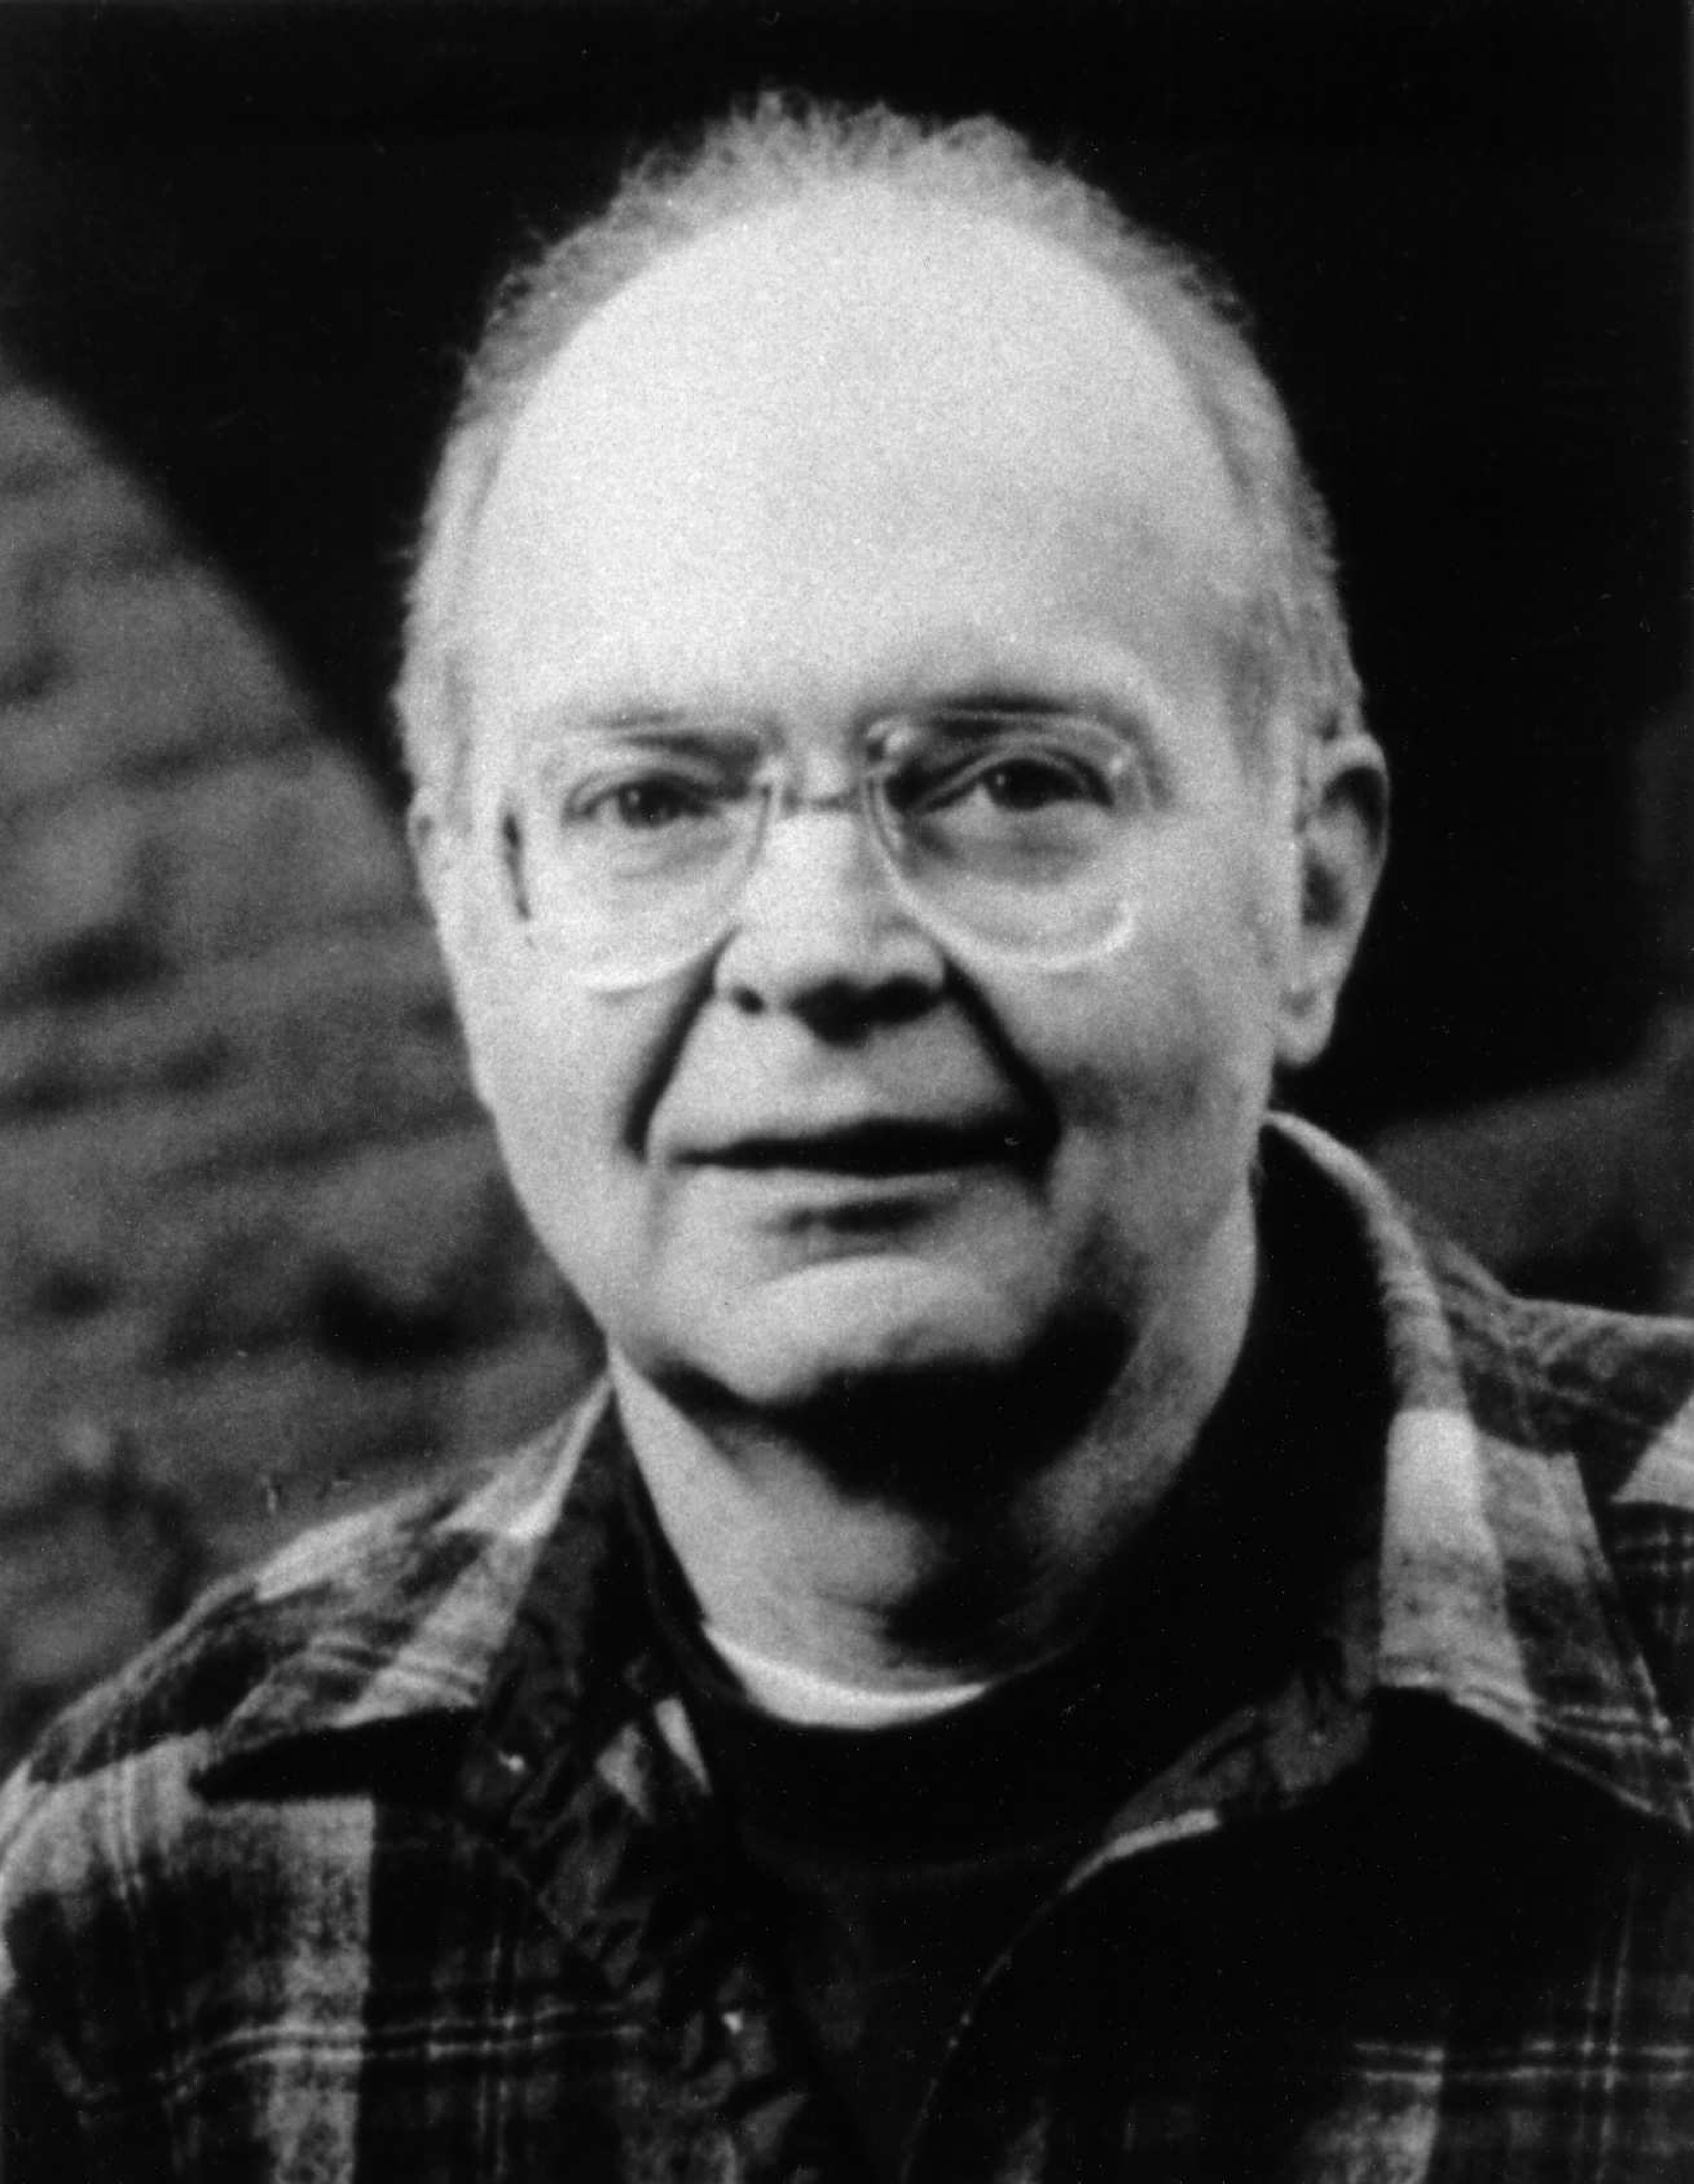
\includegraphics[height=3.0in]{don-hires}
  \caption[Donald E. Knuth, the creator of \TeX{}.]
          {Donald E. Knuth, the creator of \TeX{}.~\cite{ref:donpicture}}
  \label{fig:knuth}
\end{figure}

\LaTeX{} was designed and implemented by Leslie Lamport while he worked
at Digital Equipment Corp.  \LaTeX{} was his attempt to create a
documentation system that was easier to use than \TeX{}.  In fact,
\LaTeX{} is frequently called a ``document processor'' as opposed to a
``word processor,'' because it abstracts away the hard details of
formatting and typesetting, allowing the author to use a semantic
language to describe the output.


\section{Learning \LaTeX}
\newcommand{\us}{\hspace{-0.1ex}}
\newcommand{\teTeX}{\mbox{t\us e\us\us\TeX}}
\newcommand{\MiKTeX}{\mbox{M\us i\us K\us\us\TeX}}
%
Unfortunately, using \LaTeX{} is not quite as intuitive as using a
word processor.  However, if you invest the time in learning it, the
payoffs can be great.  Unlike a word processor, \LaTeX{} is written
like a markup language, which means you use macros\footnote{The 
SGML/HTML/XML world calls these tags.} to tell \TeX{} how to typeset
your document.  This means that you can edit your documents in any
old text editor, be it as crude as Microsoft Notepad, or something
more heavy-duty like vi\footnote{Try Vim~\cite{ref:vim} which is 
Vi Improved.}~\cite{ref:vi} or Emacs~\cite{ref:emacs}.

There are some good on-line books if you wish to learn \LaTeX{} without
having to shell out any hard earned money\footnote{You are earning money
during this work term, right?}.  The standard reference is \textit{A
not so short introduction to \LaTeXe{}}~\cite{ref:short}.  As well,
\textit{A simplified introduction to \LaTeX}~\cite{ref:simplified} is
also an excellent reference.

The fundamental resource for learning \LaTeX{} has to be \textit{\LaTeX:
a document preparation system}~\cite{ref:latex2e} which is written by
Leslie Lamport, the creator of \LaTeX.  Also of note is \textit{The
\LaTeX{} companion} which is the next step up, if you want to become a
power user.

How does one get a copy of \LaTeX?  On Unix systems, the 
\teTeX~\cite{ref:tetex} distribution is popular.  For Windows users,
\MiKTeX~\cite{ref:miktex} is the distribution of choice.  Follow each
packages installation instructions for best results\footnote{On a Debian
GNU/Linux system, invoke \texttt{aptitude~install~tetex-bin~tetex-extra}}.

You will probably want a PostScript interpreter to create PDFs or to
send PostScript output files to the printer.  You can use Adobe Distiller,
which you can purchase from Adobe Systems Inc.; or you could download
a copy of Ghostscript\footnote{Again, on Debian GNU/Linux, run
\texttt{aptitude~install~gs}}~\cite{ref:gs}.

\subsection{How \LaTeX{} works}

You create text files that include \LaTeX{} commands to generate the
final document.  You can consider it similar to writing source code
that is compiled to generate the typeset output.

Figure \ref{fig:flow} shows the control flow that a typical document
follows in order to generate PDF output.

\providecommand{\BibTeX}{\textsc{Bib}\us\TeX}
% Here is a another figure.  You MUST cite the figure in the text before 
% it appears.
%
% I draw a picture here using the picture environment.
\begin{figure}
  \centering
  \begin{picture}(300,170)
    % Draw the text boxes
    \put( 50, 150){\makebox(0,0){\fbox{\texttt{document.tex}}}}
    \put(250, 150){\makebox(0,0){\fbox{\texttt{document.bib}}}}
    \put( 50, 100){\makebox(0,0)[l]{\fbox{\texttt{document.pdf}}}}
    \put(180, 100){\makebox(0,0){\fbox{\texttt{document.aux}}}}
    \put(250,  50){\makebox(0,0){\fbox{\texttt{document.bbl}}}}
    \put(150,   0){\makebox(0,0){\fbox{\texttt{document.pdf}}}}
    % Draw the connecting lines
    \put( 75, 143){\vector( 0,-1){ 35}} % .tex -> .pdf
    \put( 75, 125){\line  ( 1, 0){105}} % .tex -> .aux
    \put(180, 125){\vector( 0,-1){ 18}} % .tex -> .aux
    \put(205,  93){\line  ( 0,-1){ 18}} % .aux -- .bbl
    \put(205,  75){\line  ( 1, 0){ 45}} % .aux -- .bbl
    \put(250, 143){\vector( 0,-1){ 86}} % .bib -> .bbl
    \put( 25, 143){\line  ( 0,-1){118}} % .tex -- .pdf
    \put(155,  93){\line  ( 0,-1){ 68}} % .aux -- .pdf
    \put(250,  43){\line  ( 0,-1){ 18}} % .bbl -- .pdf
    \put( 25,  25){\line  ( 1, 0){225}} % ------------
    \put(150,  25){\vector( 0,-1){ 18}} % .*   -> .pdf
    % Draw the text
    \put( 78, 138){\makebox(0,0)[tl]{\textsc{pdf}\LaTeX{}}}
    \put(247,  60){\makebox(0,0)[br]{\BibTeX{}}}
    \put(153,  10){\makebox(0,0)[bl]{\textsc{pdf}\LaTeX{}}}
  \end{picture}
  \caption{Control flow of a \LaTeX{} compilation.}
  \label{fig:flow}
\end{figure}

Since \LaTeX{} is a programming languages, it does have some special
characters.  Specifically, the reserved characters are: 
\verb'#',
\verb'$',
\verb'%',
\verb'&',
\verb'_',
\verb'{',
\verb'}',
\verb'~',
\verb'^',
\verb'\'.
  See Table \ref{tbl:chars} to see them in print.

% Here is a table.  You MUST cite the table in the text before it appears
% in the document.
\begin{table}
  \caption{Typesetting special characters.}
  \label{tbl:chars}
  \centering
  \begin{tabular}{|r|l|}
    \hline
    \multicolumn{1}{|c|}{\textbf{Name}} &
    \multicolumn{1}{|c|}{\textbf{Symbol}} \\
    \hline\hline
    octothorpe   & \# \\
    dollar sign  & \$ \\
    percent sign & \% \\
    ampersand    & \& \\
    underscore   & \_ \\
    left brace   & \{ \\
    right brace  & \} \\
    tilde        & \textasciitilde  \\
    circumflex   & \textasciicircum \\
    backslash    & \textbackslash   \\
    \hline
    inverted exclaimation & < \\
    inverted question     & > \\
    less than    & \textless \\
    greater than & \textgreater \\
    \hline
  \end{tabular}
\end{table}

\section{Source}

This document, and the documents it uses are available under the
GNU General Public License (GPL), reproduced in Appendix \ref{app:gnugpl}.
Note that you do not need to accept the GNU GPL to use this document, or
to use the document class.  I highly recommend that you read the GPL so
you understand your rights and privledges.

You can find the most recent version of these documents on my website
in a tarball at: \url{http://www.eng.uwaterloo.ca/~sfllaw/programs/uw-wkrpt/}.
Download the latest version, unpack it, and read the enclosed \texttt{README}
text file.

\section{To do}
There are still some things I want to do, to improve this example
document:

\begin{enumerate}
  \item Demonstrate the use of Gloss\TeX{} to create glossaries.
  \item Demonstrate the creation of an index.
  \item Look into \texttt{ieeetran.bst}.
  \item Fix all the bugs listed in Appendix \ref{app:bugs}.
\end{enumerate}

Examples that illustrate this usage are most definitely welcome.  Please
provide a patch against this document.

%%%%%%%%%%%%%%%%%%%%%%%%%%%%%%%%%%%%%%%%%%%%%%%%%%%%%%%%%%%%%%%%%%%%%
%% BACK MATTER
%%%%%%%%%%%%%%%%%%%%%%%%%%%%%%%%%%%%%%%%%%%%%%%%%%%%%%%%%%%%%%%%%%%%%
%% \backmatter will make the \section commands ignore their numbering,
\backmatter

% Here, we insert a References section, which will be formatted properly.
% The list of works you have referenced should be in FILENAME.bib,
% which will be workreport-sample.bib, if you use the command below.
%
% Note, you will need to process the document in a certain order.  First,
% run LaTeX.  The % first pass will allow LaTeX to build a list of 
% references, it may % emit warning messages such as:
%   LaTeX Warning: Reference `app:gnugpl' on page 4 undefined on input line 277.
%   LaTeX Warning: There were undefined references.
% This is normal.  Now you run BiBTeX in order to generate the proper
% layout for the references.  After this, you run LaTeX once more.
\bibliography{uw-wkrpt-bib}

%%%%%%%%%%%%%%%%%%%%%%%%%%%%%%%%%%%%%%%%%%%%%%%%%%%%%%%%%%%%%%%%%%%%%
%% APPENDICES
%%%%%%%%%%%%%%%%%%%%%%%%%%%%%%%%%%%%%%%%%%%%%%%%%%%%%%%%%%%%%%%%%%%%%
%% \appendix will reset \section numbers and turn them into letters.
%%
%% Don't forget to refer to all your appendices in the main report.
\appendix

\section{Bugs}\label{app:bugs}
Currently, there are some known problems with this document class.
\begin{itemize}
  \item It is not officially supported or acknowledged by the
        E\&CE department.
  \item Not all users have converted to using a typesetting language, and
        insist on using word processors.
  \item It does not bring world peace.
\end{itemize}

Fixes for these bugs are most certainly welcome.  Please provide a patch
against the document class document.

\section{Colophon}\label{app:colophon}
This sample document was written by Simon Law, a third-year Computer
Engineering student at the University of Waterloo, in Waterloo, ON, CA.
When he is not programming, he can be found reading or sleeping;
both of which are his favourite activities.\footnote{OK, so I don't
have a life yet.  I'm working on it.}

The best way to contact him is by e-mail, at \url{sfllaw@uwaterloo.ca}.

This document was implemented using the \texttt{ece} variant of the
\texttt{uw-wkrpt} document class.  The document class, and the 
surrounding documentation is implemented using the \LaTeXe{} macro 
package which is built on the \TeX{} typesetting system.  The documents
were generated by the web2c implementation of \TeX, found in the 
\teTeX{} distribution.  The typeface used is Computer Modern.

The entire system was written in the Vim text editor. The operating
system used was Debian GNU/Linux which ran on an IBM ThinkPad A20m. This
stalwart companion allowed him to work on this report periodically, even
during his ``off'' time up at the cottage.


\section{GNU General Public License}\label{app:gnugpl}
\renewcommand{\labelenumii}{\theenumii)}
\begin{singlespacing}
\centerline{Version 2, June 1991}

\begin{quote}
 Copyright \copyright{} 1989, 1991 Free Software Foundation, Inc.\newline
 \null\hspace{0.5in}59 Temple Place, Suite 330, Boston, 
 MA\ \ 02111-1307\ \ USA\\
 Everyone is permitted to copy and distribute verbatim copies
 of this license document, but changing it is not allowed.
\end{quote}

\subsection*{\centerline{Preamble}}

  The licenses for most software are designed to take away your
freedom to share and change it.  By contrast, the GNU General Public
License is intended to guarantee your freedom to share and change free
software--to make sure the software is free for all its users.  This
General Public License applies to most of the Free Software
Foundation's software and to any other program whose authors commit to
using it.  (Some other Free Software Foundation software is covered by
the GNU Library General Public License instead.)  You can apply it to
your programs, too.

  When we speak of free software, we are referring to freedom, not
price.  Our General Public Licenses are designed to make sure that you
have the freedom to distribute copies of free software (and charge for
this service if you wish), that you receive source code or can get it
if you want it, that you can change the software or use pieces of it
in new free programs; and that you know you can do these things.

  To protect your rights, we need to make restrictions that forbid
anyone to deny you these rights or to ask you to surrender the rights.
These restrictions translate to certain responsibilities for you if you
distribute copies of the software, or if you modify it.

  For example, if you distribute copies of such a program, whether
gratis or for a fee, you must give the recipients all the rights that
you have.  You must make sure that they, too, receive or can get the
source code.  And you must show them these terms so they know their
rights.

  We protect your rights with two steps: (1) copyright the software, and
(2) offer you this license which gives you legal permission to copy,
distribute and/or modify the software.

  Also, for each author's protection and ours, we want to make certain
that everyone understands that there is no warranty for this free
software.  If the software is modified by someone else and passed on, we
want its recipients to know that what they have is not the original, so
that any problems introduced by others will not reflect on the original
authors' reputations.

  Finally, any free program is threatened constantly by software
patents.  We wish to avoid the danger that redistributors of a free
program will individually obtain patent licenses, in effect making the
program proprietary.  To prevent this, we have made it clear that any
patent must be licensed for everyone's free use or not licensed at all.

  The precise terms and conditions for copying, distribution and
modification follow.

\subsection*{\centerline{TERMS AND CONDITIONS FOR COPYING,}\\
             \centerline{DISTRIBUTION AND MODIFICATION}}

\begin{enumerate}
\setcounter{enumi}{-1}

\item This License applies to any program or other work which contains
a notice placed by the copyright holder saying it may be distributed
under the terms of this General Public License.  The ``Program'', below,
refers to any such program or work, and a ``work based on the Program''
means either the Program or any derivative work under copyright law:
that is to say, a work containing the Program or a portion of it,
either verbatim or with modifications and/or translated into another
language.  (Hereinafter, translation is included without limitation in
the term ``modification''.)  Each licensee is addressed as ``you''.

Activities other than copying, distribution and modification are not
covered by this License; they are outside its scope.  The act of
running the Program is not restricted, and the output from the Program
is covered only if its contents constitute a work based on the
Program (independent of having been made by running the Program).
Whether that is true depends on what the Program does.

\item You may copy and distribute verbatim copies of the Program's
source code as you receive it, in any medium, provided that you
conspicuously and appropriately publish on each copy an appropriate
copyright notice and disclaimer of warranty; keep intact all the
notices that refer to this License and to the absence of any warranty;
and give any other recipients of the Program a copy of this License
along with the Program.

You may charge a fee for the physical act of transferring a copy, and
you may at your option offer warranty protection in exchange for a fee.

\item You may modify your copy or copies of the Program or any portion
of it, thus forming a work based on the Program, and copy and
distribute such modifications or work under the terms of Section 1
above, provided that you also meet all of these conditions:

  \begin{enumerate}
    \item You must cause the modified files to carry prominent notices
    stating that you changed the files and the date of any change.

    \item You must cause any work that you distribute or publish, that in
    whole or in part contains or is derived from the Program or any
    part thereof, to be licensed as a whole at no charge to all third
    parties under the terms of this License.

    \item If the modified program normally reads commands interactively
    when run, you must cause it, when started running for such
    interactive use in the most ordinary way, to print or display an
    announcement including an appropriate copyright notice and a
    notice that there is no warranty (or else, saying that you provide
    a warranty) and that users may redistribute the program under
    these conditions, and telling the user how to view a copy of this
    License.  (Exception: if the Program itself is interactive but
    does not normally print such an announcement, your work based on
    the Program is not required to print an announcement.)
  \end{enumerate}

These requirements apply to the modified work as a whole.  If
identifiable sections of that work are not derived from the Program,
and can be reasonably considered independent and separate works in
themselves, then this License, and its terms, do not apply to those
sections when you distribute them as separate works.  But when you
distribute the same sections as part of a whole which is a work based
on the Program, the distribution of the whole must be on the terms of
this License, whose permissions for other licensees extend to the
entire whole, and thus to each and every part regardless of who wrote it.

Thus, it is not the intent of this section to claim rights or contest
your rights to work written entirely by you; rather, the intent is to
exercise the right to control the distribution of derivative or
collective works based on the Program.

In addition, mere aggregation of another work not based on the Program
with the Program (or with a work based on the Program) on a volume of
a storage or distribution medium does not bring the other work under
the scope of this License.

\item You may copy and distribute the Program (or a work based on it,
under Section 2) in object code or executable form under the terms of
Sections 1 and 2 above provided that you also do one of the following:

    \begin{enumerate}
    \item Accompany it with the complete corresponding machine-readable
    source code, which must be distributed under the terms of Sections
    1 and 2 above on a medium customarily used for software interchange; or,

    \item Accompany it with a written offer, valid for at least three
    years, to give any third party, for a charge no more than your
    cost of physically performing source distribution, a complete
    machine-readable copy of the corresponding source code, to be
    distributed under the terms of Sections 1 and 2 above on a medium
    customarily used for software interchange; or,

    \item Accompany it with the information you received as to the offer
    to distribute corresponding source code.  (This alternative is
    allowed only for noncommercial distribution and only if you
    received the program in object code or executable form with such
    an offer, in accord with Subsection b above.)
    \end{enumerate}

The source code for a work means the preferred form of the work for
making modifications to it.  For an executable work, complete source
code means all the source code for all modules it contains, plus any
associated interface definition files, plus the scripts used to
control compilation and installation of the executable.  However, as a
special exception, the source code distributed need not include
anything that is normally distributed (in either source or binary
form) with the major components (compiler, kernel, and so on) of the
operating system on which the executable runs, unless that component
itself accompanies the executable.

If distribution of executable or object code is made by offering
access to copy from a designated place, then offering equivalent
access to copy the source code from the same place counts as
distribution of the source code, even though third parties are not
compelled to copy the source along with the object code.

\item You may not copy, modify, sublicense, or distribute the Program
except as expressly provided under this License.  Any attempt
otherwise to copy, modify, sublicense or distribute the Program is
void, and will automatically terminate your rights under this License.
However, parties who have received copies, or rights, from you under
this License will not have their licenses terminated so long as such
parties remain in full compliance.

\item You are not required to accept this License, since you have not
signed it.  However, nothing else grants you permission to modify or
distribute the Program or its derivative works.  These actions are
prohibited by law if you do not accept this License.  Therefore, by
modifying or distributing the Program (or any work based on the
Program), you indicate your acceptance of this License to do so, and
all its terms and conditions for copying, distributing or modifying
the Program or works based on it.

\item Each time you redistribute the Program (or any work based on the
Program), the recipient automatically receives a license from the
original licensor to copy, distribute or modify the Program subject to
these terms and conditions.  You may not impose any further
restrictions on the recipients' exercise of the rights granted herein.
You are not responsible for enforcing compliance by third parties to
this License.

\item If, as a consequence of a court judgment or allegation of patent
infringement or for any other reason (not limited to patent issues),
conditions are imposed on you (whether by court order, agreement or
otherwise) that contradict the conditions of this License, they do not
excuse you from the conditions of this License.  If you cannot
distribute so as to satisfy simultaneously your obligations under this
License and any other pertinent obligations, then as a consequence you
may not distribute the Program at all.  For example, if a patent
license would not permit royalty-free redistribution of the Program by
all those who receive copies directly or indirectly through you, then
the only way you could satisfy both it and this License would be to
refrain entirely from distribution of the Program.

If any portion of this section is held invalid or unenforceable under
any particular circumstance, the balance of the section is intended to
apply and the section as a whole is intended to apply in other
circumstances.

It is not the purpose of this section to induce you to infringe any
patents or other property right claims or to contest validity of any
such claims; this section has the sole purpose of protecting the
integrity of the free software distribution system, which is
implemented by public license practices.  Many people have made
generous contributions to the wide range of software distributed
through that system in reliance on consistent application of that
system; it is up to the author/donor to decide if he or she is willing
to distribute software through any other system and a licensee cannot
impose that choice.

This section is intended to make thoroughly clear what is believed to
be a consequence of the rest of this License.

\item If the distribution and/or use of the Program is restricted in
certain countries either by patents or by copyrighted interfaces, the
original copyright holder who places the Program under this License
may add an explicit geographical distribution limitation excluding
those countries, so that distribution is permitted only in or among
countries not thus excluded.  In such case, this License incorporates
the limitation as if written in the body of this License.

\item The Free Software Foundation may publish revised and/or new versions
of the General Public License from time to time.  Such new versions will
be similar in spirit to the present version, but may differ in detail to
address new problems or concerns.

Each version is given a distinguishing version number.  If the Program
specifies a version number of this License which applies to it and ``any
later version'', you have the option of following the terms and conditions
either of that version or of any later version published by the Free
Software Foundation.  If the Program does not specify a version number of
this License, you may choose any version ever published by the Free Software
Foundation.

\item If you wish to incorporate parts of the Program into other free
programs whose distribution conditions are different, write to the author
to ask for permission.  For software which is copyrighted by the Free
Software Foundation, write to the Free Software Foundation; we sometimes
make exceptions for this.  Our decision will be guided by the two goals
of preserving the free status of all derivatives of our free software and
of promoting the sharing and reuse of software generally.
\newcounter{Enumi}
\setcounter{Enumi}{\value{enumi}}
\end{enumerate}

\subsubsection*{\centerline{NO WARRANTY}}

\begin{enumerate}
\setcounter{enumi}{\value{Enumi}}
\item BECAUSE THE PROGRAM IS LICENSED FREE OF CHARGE, THERE IS NO WARRANTY
FOR THE PROGRAM, TO THE EXTENT PERMITTED BY APPLICABLE LAW.  EXCEPT WHEN
OTHERWISE STATED IN WRITING THE COPYRIGHT HOLDERS AND/OR OTHER PARTIES
PROVIDE THE PROGRAM ``AS IS'' WITHOUT WARRANTY OF ANY KIND, EITHER EXPRESSED
OR IMPLIED, INCLUDING, BUT NOT LIMITED TO, THE IMPLIED WARRANTIES OF
MERCHANTABILITY AND FITNESS FOR A PARTICULAR PURPOSE.  THE ENTIRE RISK AS
TO THE QUALITY AND PERFORMANCE OF THE PROGRAM IS WITH YOU.  SHOULD THE
PROGRAM PROVE DEFECTIVE, YOU ASSUME THE COST OF ALL NECESSARY SERVICING,
REPAIR OR CORRECTION.

\item IN NO EVENT UNLESS REQUIRED BY APPLICABLE LAW OR AGREED TO IN WRITING
WILL ANY COPYRIGHT HOLDER, OR ANY OTHER PARTY WHO MAY MODIFY AND/OR
REDISTRIBUTE THE PROGRAM AS PERMITTED ABOVE, BE LIABLE TO YOU FOR DAMAGES,
INCLUDING ANY GENERAL, SPECIAL, INCIDENTAL OR CONSEQUENTIAL DAMAGES ARISING
OUT OF THE USE OR INABILITY TO USE THE PROGRAM (INCLUDING BUT NOT LIMITED
TO LOSS OF DATA OR DATA BEING RENDERED INACCURATE OR LOSSES SUSTAINED BY
YOU OR THIRD PARTIES OR A FAILURE OF THE PROGRAM TO OPERATE WITH ANY OTHER
PROGRAMS), EVEN IF SUCH HOLDER OR OTHER PARTY HAS BEEN ADVISED OF THE
POSSIBILITY OF SUCH DAMAGES.
\end{enumerate}

\subsection*{\centerline{END OF TERMS AND CONDITIONS}}

\subsection*{\centerline{How to Apply These Terms to Your New Programs}}

  If you develop a new program, and you want it to be of the greatest
possible use to the public, the best way to achieve this is to make it
free software which everyone can redistribute and change under these terms.

  To do so, attach the following notices to the program.  It is safest
to attach them to the start of each source file to most effectively
convey the exclusion of warranty; and each file should have at least
the ``copyright'' line and a pointer to where the full notice is found.
% This is a hack to make the quote environment behave nicely.
\renewenvironment{quote}{\list{}{}\item\relax}{\endlist}
\begin{quote}\ttfamily\footnotesize
    \emph{one line to give the program's name and a brief 
    idea of what it\nolinebreak[4] does.}\\
    Copyright (C) \emph{year}\ \ \emph{name of author}\\
\mbox{}\\
    This program is free software; you can redistribute it and/or modify\\
    it under the terms of the GNU General Public License as published by\\
    the Free Software Foundation; either version 2 of the License, or\\
    (at your option) any later version.\\
\mbox{}\\
    This program is distributed in the hope that it will be useful,\\
    but WITHOUT ANY WARRANTY; without even the implied warranty of\\
    MERCHANTABILITY or FITNESS FOR A PARTICULAR PURPOSE.  See the\\
    GNU General Public License for more details.\\
\mbox{}\\
    You should have received a copy of the GNU General Public License\\
    along with this program; if not, write to the Free Software\\
    Foundation, Inc., 59 Temple Place, Suite 330, Boston, \\
    MA\ \ 02111-1307\ \ USA
\end{quote}


Also add information on how to contact you by electronic and paper mail.

If the program is interactive, make it output a short notice like this
when it starts in an interactive mode:
\begin{quote}\ttfamily\footnotesize
    Gnomovision version 69, Copyright (C) \emph{year}\ \ 
    \emph{name of author}\\
    Gnomovision comes with ABSOLUTELY NO WARRANTY; for details type `show w'.\\
    This is free software, and you are welcome to redistribute it\\
    under certain conditions; type `show c' for details.
\end{quote}

The hypothetical commands `show w' and `show c' should show the appropriate
parts of the General Public License.  Of course, the commands you use may
be called something other than `show w' and `show c'; they could even be
mouse-clicks or menu items--whatever suits your program.

You should also get your employer (if you work as a programmer) or your
school, if any, to sign a ``copyright disclaimer'' for the program, if
necessary.  Here is a sample; alter the names:
\begin{quote}\ttfamily\footnotesize
  Yoyodyne, Inc., hereby disclaims all copyright interest in the program\\
  `Gnomovision' (which makes passes at compilers) written by James Hacker.\\
\mbox{}\\
  \emph{signature of Ty Coon}, 1 April 1989\\
  Ty Coon, President of Vice
\end{quote}

This General Public License does not permit incorporating your program into
proprietary programs.  If your program is a subroutine library, you may
consider it more useful to permit linking proprietary applications with the
library.  If this is what you want to do, use the GNU Library General
Public License instead of this License.

\end{singlespacing}

\end{document}
